\documentclass{jsarticle}
\usepackage{amsmath}
\usepackage[dvipdfmx]{graphicx}
\usepackage{mathrsfs}
\usepackage{verbatim}
\makeatletter

\def\@thesis{機械学習特論}
\def\id#1{\def\@id{#1}}
\def\department#1{\def\@department{#1}}

\def\@maketitle{
\begin{center}
{\huge \@thesis \par} %修士論文と記載される部分
\vspace{10mm}
{\LARGE\bf \@title \par}% 論文のタイトル部分
\vspace{10mm}
{\Large \@date\par}	% 提出年月日部分
\vspace{20mm}
{\Large \@department \par}	% 所属部分
{\Large 学籍番号 \@id \par}	% 学籍番号部分
\vspace{10mm}
{\large \@author}% 氏名 
\end{center}
\par\vskip 1.5em
}

\makeatother

\title{レポート課題 1}
\date{\today}
\department{創成科学研究科 基盤科学系 情報科学コース}
\id{19-8801-009-1}
\author{北田 和}
\begin{document}
\maketitle
\newpage


\section{}

\subsection{目的}
最小二乗法の精度がどの程度のものか検討する. 

\subsection{手法}
$M$ 個のデータをランダムに生成し, 特徴量$x_i(0, 1, \dots, M)$のデータとした(ランダムさは, 正規分布に従い, これ以降使用するランダムな数字も正規分布に従う). 
これに対し, 観測データ$y_i(0, 1, \dots, M)$を式(\ref{ymake})によって作成する.
\begin{equation}
\label{ymake}
y_i = \beta \times x_i + \beta_i \times 0.5
\end{equation}
ここで, $\beta$はランダムな定数であり, $i$に関係なく一つに決める. 
一方, $\beta_i(0, 1, \dots, M)$は, $i$によって異なるランダムな数である. 
また, $x_i$に関係ないこの項はノイズに該当する. 
なお, ランダムな数は, 正規分布に従うため, 平均は0となる. 
よって, 真の関数は, 式(\ref{y}) で表すことができる. 
\begin{equation}
\label{y}
y = \beta \times x
\end{equation}
作成した特徴量$x_i$と観測データ$y_i$から, 最小二乗法によって式(\ref{y})の$\beta$を, 予測する. 
ここで, 予測した傾きを$\beta^*$, 切片を$b$とすると, 最小二乗法によって求めた, 式(\ref{y})は式(\ref{ypred})のように表せる. 
\begin{equation}
\label{ypred}
y = \beta^* \times x + b
\end{equation}


以上を計算するプログラムを以下に示す.
なお, jupyter notebookを用いて解析を行った. 



\scriptsize
\begin{verbatim}
import numpy as np
import matplotlib.pyplot as plt

Num = 100
x = np.random.randn(Num)
b = np.random.randn(1)
print(b)
y = b*x + np.random.randn(Num)*0.5
xx = np.linspace(min(x), max(x), Num)


x1 = np.full((1, Num), 1)
bm_x = np.concatenate([[x], x1])
bm_x = bm_x.T
b1 = np.dot(bm_x.T, bm_x)
print(b1)
b1 = np.linalg.inv(b1)
print(b1)
b1 = np.dot(b1, bm_x.T)
b1 = np.dot(b1, y)
print(b1)
sy = b * xx
yy = b1[0] * xx + b1[1]
plt.plot(x,y,marker='.',ls='')
print(b)
print(b1[0])
print(b1[1])
plt.plot(xx, sy, label='true line')
plt.plot(xx,yy, label='predict line')
plt.legend()
plt.savefig('')
plt.savefig('kaku.png')
\end{verbatim}
\normalsize


\subsection{結果}
生成した$\beta$は 1.262,
最小二乗法によって求めた$\beta *$は 1.237, bは, 0.027であった. 



ここで, 観測データと式(\ref{y}), 式(\ref{ypred})を図\ref{kaku}にまとめた. 横軸は特徴量 $x$ , 縦軸は観測データ$y$である. 



\begin{figure}
\begin{center}
\label{kaku}
\caption{観測データと真の解, 予測解}
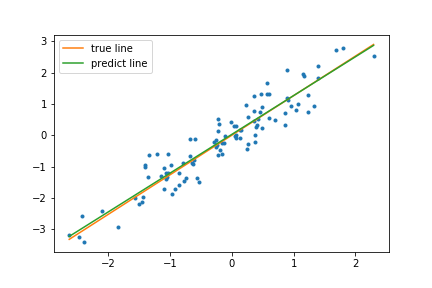
\includegraphics[width=10cm]{prog/kaku.png}
\end{center}
\end{figure}


\subsection{考察}
何度かデータを出力し直して, 傾きの誤差を確認した. 





\section{}
\subsection{目的}
リッジ回帰における正則化パラメータ$\alpha$と予測誤差の関係を調べ, 最適な$\alpha$について検討する. 

\subsection{手法}
python のライブラリである scikit-learn 内に存在する boston housing データ使用した. 
boston housing データには, 13種類の特徴量が存在する.
それぞれの特徴の構成を表\ref{boston}に示す.
これらの特徴量を用いて, 住宅価格を予測する.

\begin{table}[htb]
  \begin{center}
    \label{boston}
  \begin{tabular}{| l | l |}\hline
    カラム名  & 特徴量 \\ \hline
    CRIM & 人口 1 人当たりの犯罪発生数 \\ \hline
    ZN & 25,000 平方フィート以上の住居区画の占める割合 \\ \hline
    INDUS & 小売業以外の商業が占める面積の割合 \\ \hline
    CHAS & チャールズ川によるダミー変数 (1: 川の周辺, 0: それ以外) \\ \hline
    NOX & NOx の濃度 \\ \hline
    RM & 住居の平均部屋数 \\ \hline
    AGE & 1940 年より前に建てられた物件の割合 \\ \hline
    DIS & 5 つのボストン市の雇用施設からの距離 (重み付け済)\\ \hline
    RAD & 環状高速道路へのアクセスしやすさ \\ \hline
    TAX & $\$$10,000 ドルあたりの不動産税率の総計\\ \hline
    PTRATIO & 町毎の児童と教師の比率 \\ \hline
    B & 町毎の黒人 (Bk) の比率を次の式で表したもの。 1000(Bk $ - 0.63)^2$ \\ \hline
    LSTAT & 給与の低い職業に従事する人口の割合 (\%) \\ \hline
  \end{tabular}
  \end{center}
\end{table}


全体データのうち, ランダムな8割のデータを学習データに, 残りの2割のデータをテストデータとした.
予測誤差は, 予測の平均絶対誤差(MAE)と, 平方根平均二乗誤差(RMSE)によって導出することにした.
ここで, 予測誤差が小さくなる. つまり, MAEとRMSEが最小をとるときの, 正則化パラメータ $\alpha$ を調べることにした.
具体的には, $\alpha$ を 0 から 4.99 まで, 0.01 刻みで大きくした時の, MAEとRMSEを計算し, それぞれが, 最小をとるときの$\alpha$がどのくらいであったか調べる.
また, 以上の手順をホールドアウト法によって, 学習データとテストデータを 100 回変更した.
これにより, 導出された 100 個の $\alpha$ に対し, 平均と標準偏差を計算することで, どのようなデータでも, 予測誤差が小さくなるような $\alpha$ を検討する. 
%ここで, 正則化パラメータ$\alpha$と予測誤差の関係を調べるために, 

上記のプログラムを以下に示す. 

\clearpage
\scriptsize
\begin{verbatim}
import numpy as np
from sklearn import datasets
from sklearn import linear_model
import matplotlib.pyplot as plt
from sklearn.model_selection import train_test_split
from sklearn.metrics import accuracy_score
from sklearn.metrics import mean_squared_error
from sklearn.metrics import mean_absolute_error


boston = datasets.load_boston()

ran = 100
leng = 500


alpha = np.linspace(0, 4.99, leng)

train_score_all = np.linspace(0.001, 5, leng).reshape(1, leng)
val_score_all = np.linspace(0.001, 5, leng).reshape(1, leng)

train_mae_all = np.linspace(0.001, 5, leng).reshape(1, leng)
val_mae_all = np.linspace(0.001, 5, leng).reshape(1, leng)

train_rmse_all = np.linspace(0.001, 5, leng).reshape(1, leng)
val_rmse_all = np.linspace(0.001, 5, leng).reshape(1, leng)



for w in range(ran): 
    X_train, X_val, y_train, y_val = train_test_split(boston.data, boston.target, train_size=0.8, random_state=w)
    

    
    train_score_data = np.empty(leng, dtype=np.float)
    val_score_data = np.empty(leng, dtype=np.float)

    train_mae_data = np.empty(leng, dtype=np.float)
    val_mae_data = np.empty(leng, dtype=np.float)

    train_rmse_data = np.empty(leng, dtype=np.float)
    val_rmse_data = np.empty(leng, dtype=np.float)

    for i in range(leng) :
        clf = linear_model.Ridge(alpha = alpha[i])
        clf.fit(X_train, y_train)
    
        y_train_pred = clf.predict(X_train)
        y_val_pred = clf.predict(X_val)
    
        testy = y_val
    
        #predicted = clf.predict(boston.data)
    
        train_score_data[i] = clf.score(X_train, y_train)
        val_score_data[i] = clf.score(X_val, y_val)
        #mae = mean_absolute_error(Xtrain, y_train)
        # 平方根平均二乗誤差(RMSE)
    
        train_mae_data[i] = mean_absolute_error(y_train, y_train_pred)
        val_mae_data[i] = mean_absolute_error(y_val, y_val_pred)
    
        train_rmse_data[i] = np.sqrt(mean_squared_error(y_train, y_train_pred))
        val_rmse_data[i] = np.sqrt(mean_squared_error(y_val, y_val_pred))
        
    train_score_all = np.append(train_score_all, train_score_data.reshape(1, leng), axis=0)
    train_mae_all = np.append(train_mae_all, train_mae_data.reshape(1, leng), axis=0)
    train_rmse_all = np.append(train_rmse_all, train_rmse_data.reshape(1, leng), axis=0)
    
    val_score_all = np.append(val_score_all, val_score_data.reshape(1, leng), axis=0)
    val_mae_all = np.append(val_mae_all, val_mae_data.reshape(1, leng), axis=0)
    val_rmse_all = np.append(val_rmse_all, val_rmse_data.reshape(1, leng), axis=0)

\end{verbatim}
\normalsize

\subsection{結果}
ホールドアウト法を用いた時の, ある学習データ, テストデータに対して, MAEとRMSEは, $\alpha$の変化によって, どう変化したかを, それぞれ, 図\ref{mae_al}, \ref{rmse_al} に示す.
どちらの図をみてもわかるように, $\alpha$ が大きすぎても, 小さすぎてもMAEとRMSEは最小にはならない.

 
\begin{figure}
\begin{center}
\label{mae_al}
\caption{MAEと$\alpha$の関係}
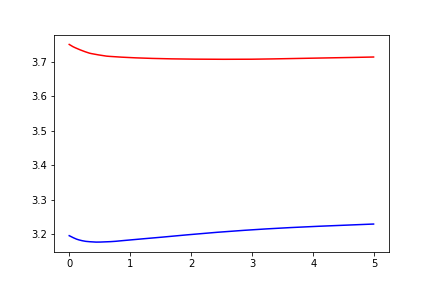
\includegraphics[width=10cm]{prog/mae.png}
\end{center}
\end{figure}



\begin{figure}
\begin{center}
\label{rmse_al}
\caption{RMSEと$\alpha$の関係}
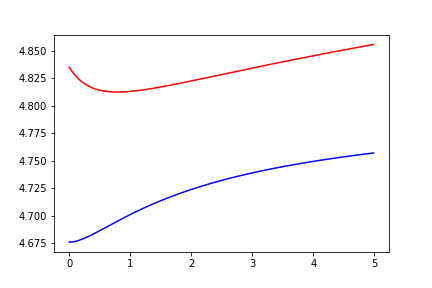
\includegraphics[width=10cm]{prog/rmse.png}
\end{center}
\end{figure}


%では, どのデータに対しても, MAEとRMSEが最小に近くなる $\alpha$ を検討するために
ホールドアウト法によって, 導出された MSEが最小となる $\alpha$ の平均は 1.18 , 
標準偏差は 1.67 となった.
一方, RMSEが最小となる $\alpha$ の平均は 0.57 , 標準偏差は 1.29 となった. 




\subsection{考察}
グラフは割愛したが, $\alpha$ が大きくなると, テストデータに対する予測誤差が学習データの予測誤差よりも大きくなる場合がみられた.
このことより, $\alpha$ が大きくなると学習データに対し, 過学習を起こす場合があると考えられる.
逆に, $\alpha$が小さい時には, 最小二乗法とあまり変わらなくなり, 予測が外れ値によってずれてしまう.
よって, $\alpha$ を検討することは重要であると考えられる. 
MSEとRMSEはそれぞれ, 真のデータに対する観測データの誤差の分布が正規分布と, ラプラス分布に従うと仮定した時の最尤推定である.
よって, $\alpha$ を検討する際は, データの取得方法をどのようにしたかも含めて検討する必要があると考えた. 


\end{document}
